\documentclass{beamer}

\mode<presentation> {
\usetheme{Madrid}
\setbeamertemplate{footline}[page number] 
\setbeamertemplate{navigation symbols}{} 
}

\usepackage{graphicx}
\usepackage{booktabs}

\renewcommand{\footnotesize}{\scriptsize}
\definecolor {processblue}{cmyk}{0.96,0,0,0}
\setbeamertemplate{frametitle}[default][center]

\title[RL Introduction]{Introduction to Reinforcement Learning} 
\author{Koganti Nishanth} 
\date{June 21, 2019}

\begin{document}

\begin{frame}
    \titlepage
\end{frame}

\begin{frame}
    \frametitle{Overview} 
    \tableofcontents 
\end{frame}

\section{Why RL?}

\begin{frame}{Branches of Machine Learning}
    \begin{figure}
        \centering
        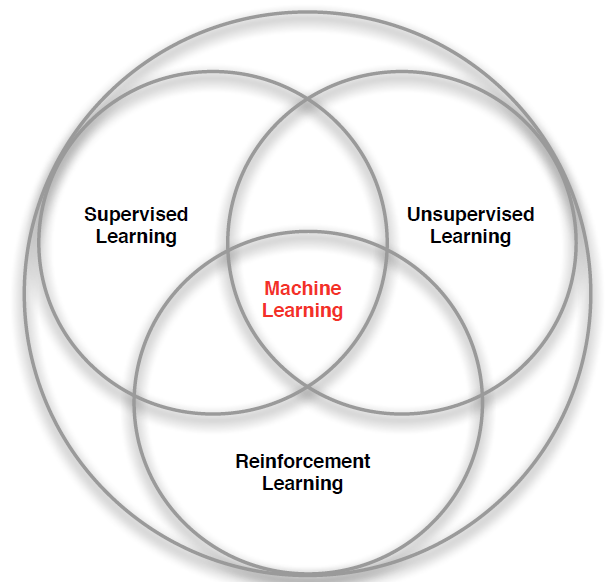
\includegraphics[width=0.65\textwidth]{images/rl_overview}
    \end{figure}
\end{frame}

\begin{frame}{Domains of Reinforcement Learning}
    \begin{figure}
        \centering
        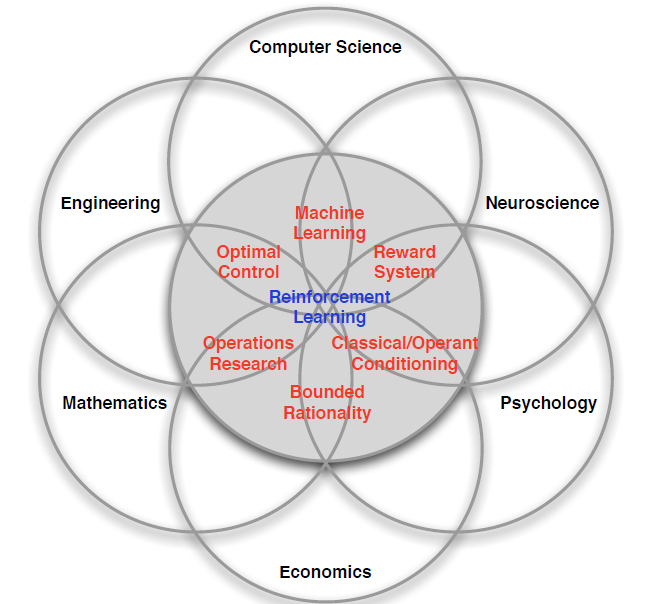
\includegraphics[width=0.65\textwidth]{images/rl_domains}
    \end{figure}    
\end{frame}

\begin{frame}{Examples of Reinforcement Learning}
    \begin{itemize}
        \item Performing stunts on an helicopter$^1$.
        \item Managing an investment portfolio.
        \item Playing atari games better than humans$^2$.
        \item Defeating world champion of Go$^3$.
        \item Performing drug discovery$^4$.
    \end{itemize}
    
    \footnotetext[1]{Abbeel, et al. ``An application of reinforcement learning to aerobatic helicopter flight.'' in \emph{NIPS 2007}.}
    \footnotetext[2]{Mnih, et al. ``Human-level control through deep reinforcement learning.'' in \emph{Nature 2015}.}
    \footnotetext[3]{Silver, et al. ``Mastering the game of Go with deep neural networks and tree search.'' in \emph{Nature 2016}.}
    \footnotetext[4]{AlphaFold 2018. Available at \url{https://deepmind.com/blog/alphafold/}}
\end{frame}

\begin{frame}{Autonomous Helicopter Flight$^1$}
    \begin{figure}
        \centering
        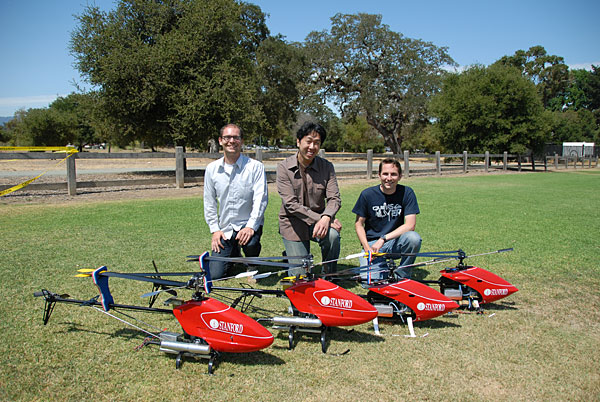
\includegraphics[width=0.7\textwidth]{images/auto_helicopter}
    \end{figure}
    
    \footnotetext[1]{Abbeel, et al. ``An application of reinforcement learning to aerobatic helicopter flight.'' in \emph{NIPS 2007}.}
\end{frame}

\section{What is RL?}

\begin{frame}{Characteristics of Reinforcement Learning}
    What makes Reinforcement Learning different?
    \begin{itemize}
        \item There is no supervision, only a \emph{reward} signal.
        \item Feedback is delayed, not instantaneous.
        \item Agent's actions effect subsequent data it receives.
    \end{itemize}
\end{frame}

\begin{frame}{Reward Hypothesis}
    Reinforcement learning is based on the \emph{reward hypothesis}:
    \begin{alertblock}{Reward Hypothesis}
        \emph{All} goals can be described by maximization of expected cumulative reward.
    \end{alertblock}
    ~\\
    Example of rewards:
    \begin{itemize}
        \item Helicopter Flight:
        \begin{itemize}
            \item Reward for following desired trajectory.
            \item Punishment for crashing.
        \end{itemize}
        
        \item Play Atari games:
        \begin{itemize}
            \item Reward/punishment for increasing/decreasing score.
        \end{itemize}
    \end{itemize}
\end{frame}

\begin{frame}{Agent and Environment}
    \begin{columns}
        \begin{column}{0.5\textwidth}
            \begin{figure}
                \centering
                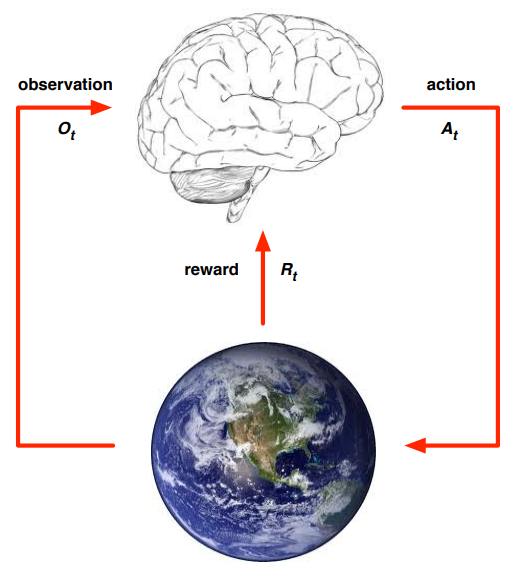
\includegraphics[width=\textwidth]{images/agent_env}
            \end{figure}        
        \end{column}
        
        \begin{column}{0.5\textwidth}
            \begin{itemize}
                \item At each step $t$, the agent:
                \begin{itemize}
                    \item Executes action $a_t$.
                    \item Receives states $s_t$.
                    \item Receives scalar reward $r_t$.\\~
                \end{itemize}
                
                \item The environment:
                \begin{itemize}
                    \item Receives action $a_t$.
                    \item Emits observation $s_{t+1}$.
                    \item Emits scalar reward $r_{t+1}$.
                \end{itemize}
            \end{itemize}
        \end{column}
    \end{columns}
\end{frame}

\section{Components}

\begin{frame}{Major Components of RL Agents}
    \begin{itemize}
        \item RL Agent may include following components:\\~
        \begin{itemize}
            \item Policy: Agent's behavior function.\\~
            \item Value function: Utility of each state and/or action.\\~
            \item Model: Agent's representation of the environment.
        \end{itemize}
    \end{itemize}
\end{frame}

\begin{frame}{Policy}
    \begin{itemize}
        \item A \emph{policy} models the agent's behavior.
        \item Function from state to action.
        \item Deterministic policy: $a = \pi(s)$.
        \item Stochastic policy: $\pi(a|s) = \mathbb{P}[a_t=a|s_t=s]$.
    \end{itemize}
    
    \begin{figure}
        \centering
        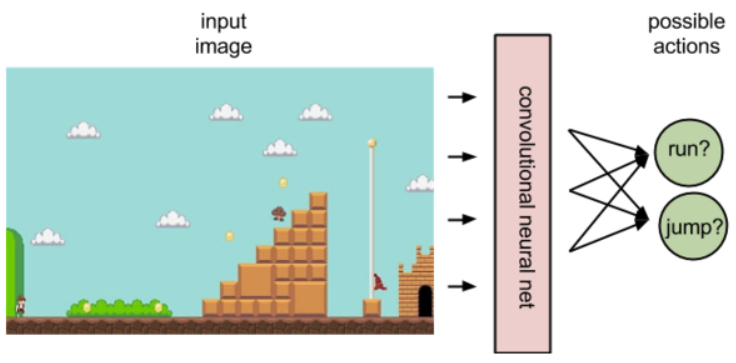
\includegraphics[width=0.8\textwidth]{images/policy_func}
    \end{figure}
\end{frame}

\begin{frame}{Value Function}
    \begin{itemize}
        \item Value function is a prediction of future reward.
        \item Used to evaluate the goodness/badness of states.
        \item Select between actions using this value function.
    \end{itemize}    
    
    \begin{equation*}
        v_{\pi}(s) = \mathbb{E}_{\pi}[r_{t+1} + \gamma r_{t+2} + \gamma^2 r_{t+3} + \cdots | s_t=s]
    \end{equation*}
    
    \begin{figure}
        \centering
        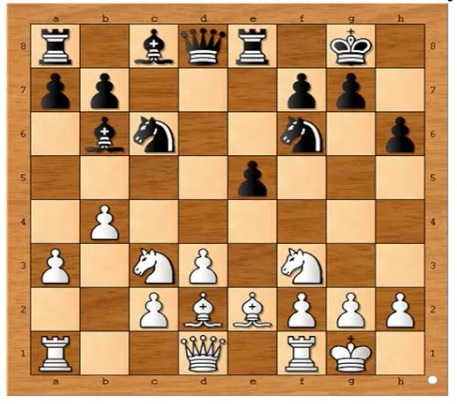
\includegraphics[width=0.4\textwidth]{images/chess_value}
    \end{figure}
    \centering Is this a good state for white?
\end{frame}

\begin{frame}{Model}
    \begin{itemize}
        \item A \emph{model} predicts what the environment will do next
        \item $\mathcal{P}$ predicts the next state
        \item $\mathcal{R}$ predicts the next reward
    \end{itemize}
    
    \begin{equation*}
        \mathcal{P}^a_{ss'} = \mathbb{P}[s_{t+1} = s' | s_t=s, a_t=a]
    \end{equation*}
    
    \begin{equation*}
        \mathcal{R}^a_s = \mathbb{R}[r_{t+1} | s_t=s, a_t=a]
    \end{equation*}
\end{frame}

\begin{frame}{Taxonomy of RL Algorithms}
    \begin{figure}
        \centering
        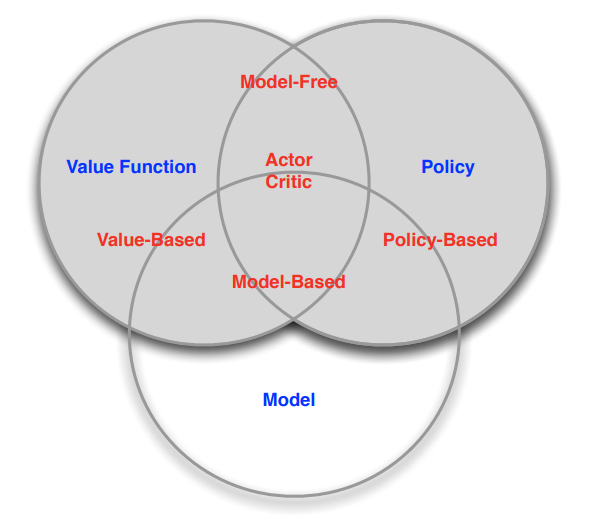
\includegraphics[width=0.7\textwidth]{images/rl_taxonomy}
    \end{figure}
\end{frame}

\section{Examples}

\begin{frame}{Maze Example}
    \begin{columns}
        \begin{column}{0.5\textwidth}
            \begin{figure}
                \centering
                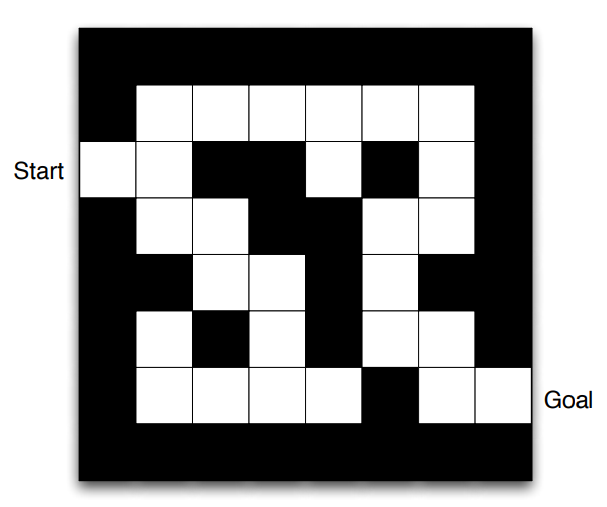
\includegraphics[width=\textwidth]{images/maze_eg}
            \end{figure}
        \end{column}
        
        \begin{column}{0.5\textwidth}
            \begin{itemize}
                \item Rewards: -1 per time step.
                \item Actions: N,S,E,W.
                \item State: Agent's position on maze.
            \end{itemize}
        \end{column}
    \end{columns}
\end{frame}

\begin{frame}{Maze Example: Policy}
    \begin{figure}
        \centering
        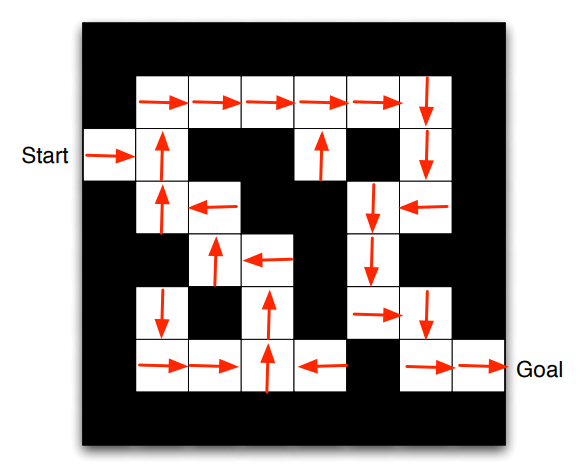
\includegraphics[width=0.7\textwidth]{images/maze_policy}
    \end{figure}
    
    \centering Red arrows indicate actions taken as per policy.
\end{frame}

\begin{frame}{Maze Example: Value Function}
    \begin{figure}
        \centering
        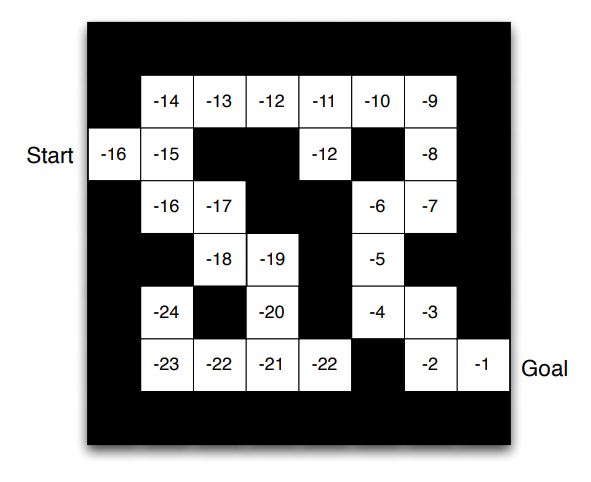
\includegraphics[width=0.7\textwidth]{images/maze_value}
    \end{figure}
    
    \centering Numbers in grid indicate expected \emph{long-term} rewards for that cell.
\end{frame}

\begin{frame}{Maze Example: Model}
    \begin{figure}
        \centering
        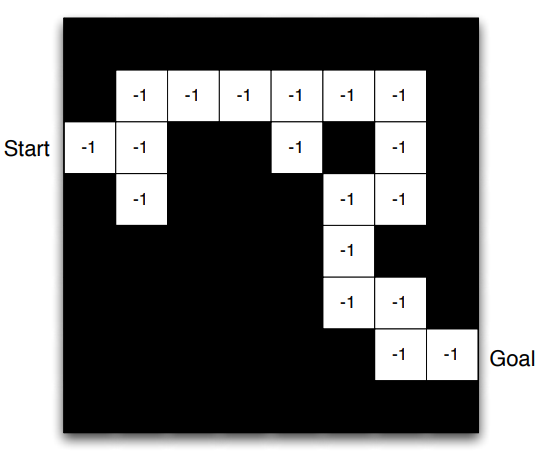
\includegraphics[width=0.65\textwidth]{images/maze_model}
    \end{figure}
    
    \centering $\mathcal{P}^{a}_{ss'}$ and $\mathcal{R}^{a}_{s}$ are shown by grid and numbers. \\ Note: Model can be imperfect!
\end{frame}

\begin{frame}{Case Study: Atari Game Play}
    \begin{columns}
        \begin{column}{0.5\textwidth}
            \begin{figure}
                \centering
                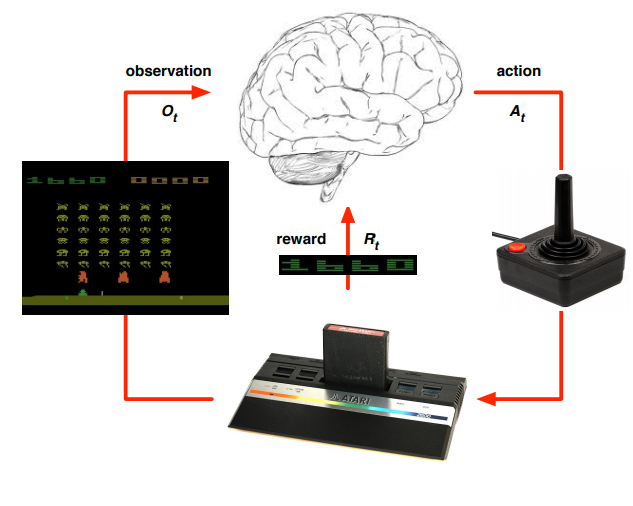
\includegraphics[width=\textwidth]{images/atari_env}
            \end{figure}
        \end{column}
        
        \begin{column}{0.5\textwidth}
            \begin{itemize}
                \item Learn directly from interactive game play.
                \item Relies on value function based RL.
                \item Approximate value function using deep neural network.
            \end{itemize}
        \end{column}
    \end{columns}
    
    \footnotetext[1]{Mnih, et al. ``Human-level control through deep reinforcement learning.'' in \emph{Nature 2015}.}
\end{frame}

\section{Resources}

\begin{frame}{Tutorials for RL}
    \begin{itemize}
        \item Andrew Ng: CS 229 Course Lectures 16-20$^1$.\\~
        \item David Silver: Reinforcement Learning Course$^2$.\\~
        \item Spinning up with Deep Reinforcement Learning: OpenAI$^3$.
        
        \footnotetext[1]{\url{https://www.youtube.com/watch?v=UzxYlbK2c7E}}
        \footnotetext[2]{\url{http://www0.cs.ucl.ac.uk/staff/d.silver/web/Teaching.html}}
        \footnotetext[3]{\url{https://spinningup.openai.com/en/latest/}}
    \end{itemize}
\end{frame}

\begin{frame}{Software Resources}
    \begin{itemize}
        \item Awesome Reinforcement Learning: {github.com/aikorea/awesome-rl}.\\~
        \item OpenAI Gym: \url{github.com/openai/gym}.
        \item Unity ML: \url{github.com/Unity-Technologies/ml-agents}.\\~
        \item garage: \url{github.com/rlworkgroup/garage}.
        \item trfl: \url{github.com/deepmind/trfl/}.
        
    \end{itemize}
\end{frame}

\begin{frame}[noframenumbering]
\Huge{\centerline{Thank You}}
\end{frame}

\end{document}

